% !TEX program = xelatex
\documentclass[a4paper,12pt]{article}

\usepackage{fontspec}
\usepackage[a4paper,margin=2.6cm]{geometry}
\usepackage{array}
\usepackage{amsmath}
\usepackage{amssymb}
\usepackage{booktabs}
\usepackage{tabularx}
\usepackage{enumitem}
\usepackage{hyperref}
\usepackage{xcolor}
\usepackage{setspace}
\usepackage{titlesec}
\usepackage{algorithm}
\usepackage{algpseudocode}
\usepackage{tikz}

\usetikzlibrary{arrows.meta,positioning,fit,calc,shapes.geometric,shapes.multipart}

\setmainfont{Noto Serif CJK SC}
\setsansfont{Noto Sans CJK SC}
\setmonofont{DejaVu Sans Mono}

\XeTeXlinebreaklocale "zh"
\XeTeXlinebreakskip = 0pt plus 1pt

\hypersetup{
  colorlinks=true,
  linkcolor=black,
  urlcolor=black,
  pdftitle={ForL0 State Backend 设计说明书 v2.0}
}

\renewcommand{\contentsname}{目\quad 录}
\renewcommand{\tablename}{表}
\renewcommand{\figurename}{图}
\floatname{algorithm}{算法}

\algrenewcommand\algorithmicrequire{\textbf{输入：}}
\algrenewcommand\algorithmicensure{\textbf{输出：}}

\setstretch{1.25}
\setlength{\parindent}{2em}
\setlength{\parskip}{0.3em}
\setlength{\emergencystretch}{3em}
\sloppy

\setlist[itemize]{leftmargin=2em,itemsep=0.2em,topsep=0.3em}
\setlist[enumerate]{leftmargin=2.2em,itemsep=0.2em,topsep=0.3em}

\titleformat{\section}{\large\bfseries}{\thesection.}{0.6em}{}
\titleformat{\subsection}{\normalsize\bfseries}{\thesubsection}{0.6em}{}
\titleformat{\subsubsection}{\normalsize\bfseries}{\thesubsubsection}{0.6em}{}

\newcommand{\project}{ForL0 State Backend}

\definecolor{figblue}{RGB}{236,242,255}
\definecolor{figgreen}{RGB}{235,247,238}
\definecolor{figorange}{RGB}{250,241,231}
\definecolor{figgray}{RGB}{248,249,251}
\definecolor{figline}{RGB}{85,85,85}

\tikzset{
  controlbox/.style={draw=black!55, rounded corners=4pt, line width=0.6pt, fill=figblue, minimum height=0.95cm, inner xsep=7pt, inner ysep=5pt, align=center, font=\footnotesize\sffamily},
  bridgebox/.style={draw=black!55, rounded corners=4pt, line width=0.6pt, fill=figorange, minimum height=0.95cm, inner xsep=7pt, inner ysep=5pt, align=center, font=\footnotesize\sffamily},
  databox/.style={draw=black!55, rounded corners=4pt, line width=0.6pt, fill=figgreen, minimum height=0.95cm, inner xsep=7pt, inner ysep=5pt, align=center, font=\footnotesize\sffamily},
  neutralbox/.style={draw=black!55, rounded corners=4pt, line width=0.6pt, fill=white, minimum height=0.95cm, inner xsep=7pt, inner ysep=5pt, align=center, font=\footnotesize\sffamily},
  panel/.style={draw=black!30, rounded corners=7pt, line width=0.55pt, fill=figgray},
  ctrlcell/.style={draw=black!55, line width=0.45pt, fill=figblue, minimum width=0.38cm, minimum height=0.38cm, inner sep=0pt},
  keycell/.style={draw=black!55, line width=0.45pt, fill=figorange, minimum width=0.40cm, minimum height=0.46cm, inner sep=0pt},
  valuecell/.style={draw=black!55, line width=0.45pt, fill=figgreen, minimum width=0.40cm, minimum height=0.46cm, inner sep=0pt},
  hashcell/.style={draw=black!55, line width=0.45pt, fill=yellow!20, minimum width=0.40cm, minimum height=0.46cm, inner sep=0pt},
  barseg/.style={draw=black!55, line width=0.45pt, minimum height=0.78cm, inner sep=0pt, align=center, font=\footnotesize\sffamily},
  line/.style={-{Latex[length=1.9mm]}, draw=figline, line width=0.65pt},
  figtitle/.style={font=\small\sffamily\bfseries, text=black!82},
  figlabel/.style={font=\footnotesize\sffamily, text=black!78}
}

\begin{document}

\begin{titlepage}
\centering
\vspace*{3cm}

{\LARGE\bfseries \project 设计说明书\par}
\vspace{1.2cm}
{\Large v2.0\par}

\vspace{3.5cm}

\begin{tabular}{rl}
文档类型： & 项目交付文档 \\
文档属性： & 设计说明书 \\
适用对象： & 项目评审、研发交接、交付验收 \\
版本日期： & 2026年4月 \\
\end{tabular}

\vfill

{\large 项目名称：\project\par}
\end{titlepage}

\tableofcontents
\newpage

\section{整体架构设计}

\project{} 面向 Apache Flink 的 Keyed State 场景设计，目标是在保持 Flink 状态接口、命名空间语义和 Checkpoint 机制兼容的前提下，将状态访问的主要数据路径收敛到一套原生状态引擎中，通过类型特化、缓存友好的哈希组织和低复制快照机制，降低状态访问延迟并提升整体处理效率。

与早期版本相比，当前实现已经从“Java 侧分层 StateStore 主导”的结构演进为“Java 控制层 + JNI 桥接层 + C++ 原生状态引擎”的三层架构。Java 层承担接口适配、状态注册和用户函数执行，native 层承担状态组织、命名空间隔离、哈希存储以及快照恢复。本文档仅说明系统设计本身，不再展开构建、部署和配置细节；相关内容由《编译构建指导书》和《使用说明书》单独说明。

\subsection{总体架构}

系统围绕 \texttt{StateEngine -> StateTable -> KeyGroup -> Namespace -> SwissTable} 的层级展开。一个任务实例对应一个 native \texttt{StateEngine}；每个状态描述符在 native 侧注册为一个 typed \texttt{StateTable<K,V>}；每个 \texttt{StateTable} 再按 key-group 和 namespace 组织具体状态条目；最底层的键值映射由 \texttt{SwissTable<K,V>} 完成。

整体职责可概括如下：

\begin{itemize}
  \item Java 控制层负责与 Flink 运行时对接，管理状态对象生命周期、serializer 分析、状态注册和快照调度。
  \item JNI 桥接层负责共享库装载、handle 透传以及按类型划分的 native 调用入口。
  \item C++ 原生数据层负责状态条目的权威存储、哈希组织、命名空间管理、Copy-On-Write 快照和恢复写入。
\end{itemize}

这一结构的关键意义在于，状态主数据面已经完全位于 native 侧，Java 层不再维护一套独立的状态表副本，也不再承担状态快照的主序列化职责。

\subsection{状态访问优化路径}

系统专门设计了一层状态访问优化路径，用于缩短热点场景上的分支判断、对象封装和序列化链路。该优化路径不是独立的表结构，而是由以下机制共同构成：

\begin{itemize}
  \item Java 状态对象在初始化阶段预计算访问策略，将 key、namespace 与 value 的组合固化为固定分支。
  \item \texttt{NativeEngine} 按高频类型组合暴露窄接口，例如 long key、int key、TimeWindow namespace、typed inner map 等专用路径。
  \item RowData key 通过 \texttt{RowDataKeyAccessor} 识别为单字段 primitive、固定长度多字段或 generic bytes 三类编码方式。
  \item 对部分 BinaryRowData 或 bytes value，native 层支持零拷贝读取，减少中间 \texttt{byte[]} 和对象重建成本。
\end{itemize}

因此，系统的性能优化重点并不是改变 Flink 状态语义，而是在保持语义不变的前提下，尽量让热点访问路径走最短 JNI 路由、最窄类型表示和最少数据复制。

\subsection{原生状态表组织}

当前实现中，负责权威状态存储的核心结构是 native 侧的 \texttt{StateTable<K,V>} 与其内部的 \texttt{SwissTable<K,V>}。Java 层通过状态名、serializer 和类型布局将状态注册到 native 层，后续所有读写、清理、遍历和恢复都通过 state handle 回到对应的 \texttt{StateTable}。

状态表组织遵循以下规则：

\begin{itemize}
  \item 每个 Flink 状态描述符在 \texttt{StateEngine} 中对应唯一的 state handle。
  \item 每个 state handle 对应一张 typed \texttt{StateTable<K,V>}。
  \item 每张 \texttt{StateTable} 按 key-group 划分内部状态分区，与 Flink key-group 路由模型一致。
  \item VoidNamespace 场景下直接访问 key-group 对应的 \texttt{SwissTable}；一般 namespace 场景下先路由到 namespace，再进入该 namespace 独立持有的 \texttt{SwissTable}。
\end{itemize}

这种组织方式同时满足了状态隔离、快照遍历稳定性和恢复写入粒度的要求，是整个后端一致性与可恢复性的基础。

\begin{figure}[htbp]
\centering
\begin{tikzpicture}[x=1cm,y=1cm]
  \node[panel, minimum width=11.6cm, minimum height=1.2cm] (lane0) at (8.75,7.05) {};
  \node[panel, minimum width=11.6cm, minimum height=1.45cm] (lane1) at (8.75,5.25) {};
  \node[panel, minimum width=11.6cm, minimum height=1.15cm] (lane2) at (8.75,3.45) {};
  \node[panel, minimum width=11.6cm, minimum height=2.15cm] (lane3) at (8.75,1.05) {};

  \node[figtitle, anchor=west, font=\footnotesize\sffamily\bfseries, fill=white, inner xsep=2pt, inner ysep=1pt, text width=2.2cm, align=left] at (0.25,7.05) {Flink 运行时};
  \node[figtitle, anchor=west, font=\footnotesize\sffamily\bfseries, fill=white, inner xsep=2pt, inner ysep=1pt, text width=2.2cm, align=left] at (0.25,5.25) {Java 控制层};
  \node[figtitle, anchor=west, font=\footnotesize\sffamily\bfseries, fill=white, inner xsep=2pt, inner ysep=1pt, text width=2.2cm, align=left] at (0.25,3.45) {JNI 桥接层};
  \node[figtitle, anchor=west, font=\footnotesize\sffamily\bfseries, fill=white, inner xsep=2pt, inner ysep=1pt, text width=2.2cm, align=left] at (0.25,1.05) {原生数据层};

  \node[controlbox, minimum width=5.5cm] (flink) at (8.75,7.05) {Runtime / State API / Checkpoint};

  \node[controlbox, minimum width=2.55cm] (factory) at (5.15,5.25) {StateBackend\\Factory};
  \node[controlbox, minimum width=2.65cm] (backend) at (8.75,5.25) {Keyed\\Backend};
  \node[controlbox, minimum width=2.75cm] (typeacc) at (12.2,5.25) {Type Analyzer\\RowData Path};

  \node[bridgebox, minimum width=3.0cm] (jni) at (8.75,3.45) {NativeEngine\\Typed JNI};

  \node[databox, minimum width=1.95cm] (engine) at (4.2,1.05) {StateEngine};
  \node[databox, minimum width=2.0cm] (table) at (6.45,1.05) {StateTable};
  \node[databox, minimum width=2.2cm] (route) at (8.75,1.05) {KeyGroup /\\Namespace};
  \node[databox, minimum width=1.95cm] (swiss) at (11.15,1.05) {SwissTable};
  \node[neutralbox, minimum width=2.05cm] (snapshot) at (13.35,1.05) {Snapshot /\\Restore / COW};

  \draw[line] (flink.south) -- (backend.north);
  \draw[line] (factory.east) -- (backend.west);
  \draw[line] (typeacc.west) -- (backend.east);
  \draw[line] (backend.south) -- (jni.north);
  \draw[line] (jni.south) -- (route.north);
  \draw[line] (engine.east) -- (table.west);
  \draw[line] (table.east) -- (route.west);
  \draw[line] (route.east) -- (swiss.west);
  \draw[line] (swiss.east) -- (snapshot.west);
\end{tikzpicture}
\caption{整体架构图}
\end{figure}

\subsection{组件解耦与集成}

\project{} 的组件划分遵循“控制面与数据面分离”的原则。Flink 侧接口、Java 状态适配、JNI 桥接和 native 数据结构各自有明确职责边界，从而保证底层存储结构可以独立优化，而不破坏上层状态接口语义。

核心组件的职责关系如下：

\begin{itemize}
  \item \texttt{ForL0StateBackend} 与 \texttt{ForL0StateBackendFactory}：负责 Flink 侧后端创建与插件注册。
  \item \texttt{ForL0KeyedStateBackendBuilder}：负责 native 引擎创建、状态恢复初始化和 backend 实例构建。
  \item \texttt{ForL0KeyedStateBackend}：负责管理 engine handle、state handle、状态对象缓存以及快照协调。
  \item \texttt{NativeEngine}：负责定义 JNI 接口并承担共享库加载。
  \item \texttt{TypeAnalyzer} 与 \texttt{RowDataKeyAccessor}：负责类型识别、布局描述生成和 RowData 快路径支持。
  \item \texttt{StateEngine}、\texttt{StateTable} 与 \texttt{SwissTable}：共同构成 native 数据面，承担状态组织、访问、快照和恢复。
\end{itemize}

\begin{figure}[htbp]
\centering
\begin{tikzpicture}[x=1cm,y=1cm]
  \node[panel, minimum width=11.8cm, minimum height=3.1cm] (javaPanel) at (8.75,3.72) {};
  \node[panel, minimum width=6.3cm, minimum height=1.55cm] (nativePanel) at (8.75,0.35) {};

  \node[figtitle, anchor=west, font=\footnotesize\sffamily\bfseries, fill=white, inner xsep=2pt, inner ysep=1pt, text width=2.2cm, align=left] at (0.45,5.05) {Java 控制面};
  \node[figtitle, anchor=west, font=\footnotesize\sffamily\bfseries, fill=white, inner xsep=2pt, inner ysep=1pt, text width=2.2cm, align=left] at (0.45,0.35) {原生数据面};

  \node[controlbox, minimum width=2.15cm] (builder) at (5.0,4.1) {Backend\\Builder};
  \node[controlbox, minimum width=2.35cm] (backend2) at (8.75,4.1) {Keyed\\Backend};
  \node[controlbox, minimum width=2.55cm] (type2) at (12.3,4.1) {Type Analyzer\\RowData Path};

  \node[controlbox, minimum width=2.0cm] (stateobj2) at (4.95,2.72) {State\\Objects};
  \node[controlbox, minimum width=1.9cm] (pq2) at (7.15,2.72) {Priority\\Queue};
  \node[controlbox, minimum width=2.1cm] (snapshot2) at (11.05,2.72) {Snapshot\\Strategy};

  \node[bridgebox, minimum width=2.2cm] (native2) at (8.75,1.42) {Native\\Engine};
  \node[databox, minimum width=2.0cm] (engine4) at (7.4,0.35) {StateEngine};
  \node[databox, minimum width=2.35cm] (table4) at (10.3,0.35) {StateTable /\\SwissTable};

  \coordinate (hub2) at (8.75,3.35);

  \draw[line] (builder.east) -- (backend2.west);
  \draw[line] (type2.west) -- (backend2.east);
  \draw[line] (backend2.south) -- (hub2);
  \draw[line] (hub2) -| (stateobj2.north);
  \draw[line] (hub2) -| (pq2.north);
  \draw[line] (hub2) -| (snapshot2.north);
  \draw[line] (hub2) -- (native2.north);
  \draw[line] (pq2.south) |- (native2.west);
  \draw[line] (snapshot2.south) |- (native2.east);
  \draw[line] (native2.south) -- ++(0,-0.22) -| (engine4.north);
  \draw[line] (engine4.east) -- (table4.west);
\end{tikzpicture}
\caption{ForL0StateBackend 组件图}
\end{figure}

\section{架构设计细节}

\project{} 遵循 Flink \texttt{AbstractStateBackend} 与 \texttt{AbstractKeyedStateBackend} 的扩展方式。Java 层围绕状态描述符、serializer 和运行时上下文选择访问路径；native 层围绕 \texttt{StateTable<K,V>} 与 \texttt{SwissTable<K,V>} 组织读写、快照导出和恢复重建。

\subsection{可复用组件与扩展组件}

当前实现并不是完全绕开 Flink 原有状态框架，而是在与状态后端集成、优先队列管理、快照元信息和状态接口层面复用 Flink 的成熟机制，并将 Keyed State 的主数据路径替换为 ForL0 自身的 native 实现。

\subsubsection{ForL0StateBackend 与 ForL0KeyedStateBackend}

\texttt{ForL0StateBackend} 是 Flink 侧的后端入口，负责创建具体的 \texttt{ForL0KeyedStateBackendBuilder}。\texttt{ForL0KeyedStateBackend} 则是 Java 壳层中的核心控制组件，承担以下职责：

\begin{itemize}
  \item 持有 native engine handle 和各状态的 native state handle。
  \item 缓存已创建状态对象与 state meta info。
  \item 在状态首次使用时完成 serializer 兼容性校验与 native 状态注册。
  \item 创建五类 Flink 状态实现，并把状态操作映射为相应 JNI 调用。
\end{itemize}

它在结构上是 Java 控制层与 native 数据层的直接衔接点，在语义上是 Flink 原生 KeyedStateBackend 的兼容实现。

\subsubsection{PriorityQueueManager / HeapPriorityQueue}

定时器与优先队列部分继续沿用 Flink 原生实现。\project{} 不改变优先队列内部行为与定时器语义，只替换主状态的键值存储路径。因此，Priority Queue 状态仍按照 Flink 既有方式参与快照和恢复。

\subsubsection{NativeEngine}

\texttt{NativeEngine} 是 Java 层访问原生状态引擎的统一入口。该组件一方面负责共享库装载，另一方面定义 Java 到 C++ 的函数映射。其核心职责包括：

\begin{itemize}
  \item 提供 \texttt{createEngine}、\texttt{destroyEngine} 等生命周期接口。
  \item 提供状态注册接口，用于在 native 层创建 typed \texttt{StateTable}。
  \item 提供 ValueState、ListState、MapState、ReducingState、AggregatingState 的 typed 访问接口。
  \item 提供快照准备、数据导出、数据恢复和快照释放接口。
\end{itemize}

当前实现中，JNI 层不保存状态本体，但它定义了 Java 控制层访问 native 数据面的全部入口。

\subsection{关键设计组件}

\subsubsection{StateEngine}

\texttt{StateEngine} 是 native 数据面的最顶层组件，负责管理所有已注册状态的句柄和状态表实例。JNI 接收到一次状态访问时，先根据 state handle 找到对应 \texttt{StateTable}，再结合 key-group 和 namespace 路由到最终的 \texttt{SwissTable}。

在快照阶段，\texttt{StateEngine} 统一触发所有状态表进入或退出 Copy-On-Write 视图，从而保证同一次 checkpoint 周期内整套状态共享一致的快照边界。

\subsubsection{状态布局与命名空间组织}

状态条目在 native 侧围绕状态表、key-group、namespace 和 \texttt{SwissTable} 展开。其设计要点如下：

\begin{itemize}
  \item 对于 VoidNamespace，每个 key-group 直接对应一张 \texttt{SwissTable<K,V>}，访问路径最短。
  \item 对于一般 namespace，每个 key-group 下维护 namespace 到 \texttt{SwissTable<K,V>} 的映射，不同 namespace 的条目不混放在同一张表中。
  \item 当某个 namespace 在删除后已经为空时，系统及时移除对应空表，避免长期保留无效容器。
\end{itemize}

这种组织方式使得 checkpoint 导出、restore 重建和 namespace merge 都可以围绕统一的数据结构完成。

\begin{figure}[htbp]
\centering
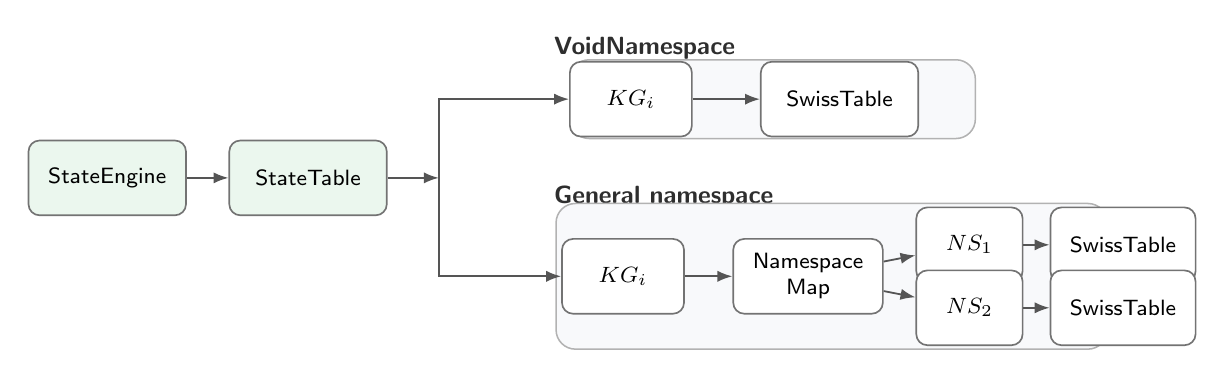
\begin{tikzpicture}[x=1cm,y=1cm]
  \node[databox, minimum width=2.0cm] (engine3) at (1.9,2.0) {StateEngine};
  \node[databox, minimum width=2.0cm] (statea) at (4.45,2.0) {StateTable};

  \node[figtitle, anchor=west] at (7.45,3.65) {VoidNamespace};
  \node[panel, minimum width=5.15cm, minimum height=1.0cm] (voidPanel) at (10.35,3.0) {};
  \node[neutralbox, minimum width=1.55cm] (kg0) at (8.55,3.0) {$KG_i$};
  \node[neutralbox, minimum width=2.0cm] (voidns) at (11.2,3.0) {SwissTable};

  \node[figtitle, anchor=west] at (7.45,1.75) {General namespace};
  \node[panel, minimum width=7.0cm, minimum height=1.85cm] (genPanel) at (11.1,0.75) {};
  \node[neutralbox, minimum width=1.55cm] (kg1) at (8.45,0.75) {$KG_i$};
  \node[neutralbox, minimum width=1.9cm] (nsmap) at (10.8,0.75) {Namespace\\Map};
  \node[neutralbox, minimum width=1.35cm] (ns1) at (12.85,1.15) {$NS_1$};
  \node[neutralbox, minimum width=1.35cm] (ns2) at (12.85,0.35) {$NS_2$};
  \node[neutralbox, minimum width=1.8cm] (nsTable1) at (14.8,1.15) {SwissTable};
  \node[neutralbox, minimum width=1.8cm] (nsTable2) at (14.8,0.35) {SwissTable};

  \draw[line] (engine3) -- (statea);
  \draw[line] (statea.east) -- ++(0.65,0) coordinate (branch);
  \draw[line] (branch) |- (kg0.west);
  \draw[line] (branch) |- (kg1.west);
  \draw[line] (kg0) -- (voidns);
  \draw[line] (kg1) -- (nsmap);
  \draw[line] (nsmap) -- (ns1);
  \draw[line] (nsmap) -- (ns2);
  \draw[line] (ns1) -- (nsTable1);
  \draw[line] (ns2) -- (nsTable2);
\end{tikzpicture}
\caption{原生状态组织结构图}
\end{figure}

\subsubsection{SwissTable}

\texttt{SwissTable<K,V>} 是状态系统的底层哈希存储结构，负责维护键到值的高效映射。其设计要点包括：

\begin{itemize}
  \item 采用 ctrl byte 加连续 slot 布局。
  \item 采用 \(H_1\) / \(H_2\) 哈希位分配方式，其中 \(H_2\) 写入 ctrl 字节，\(H_1\) 用于探测起点。
  \item 按 group 扫描 ctrl 区，先过滤候选槽位，再执行键比较。
  \item 使用 2 的幂容量、tombstone 删除和 grow/rehash 机制整理表布局。
  \item 命中后直接在 slot 中读取 value，不再经过额外的值地址层。
\end{itemize}

这意味着 \texttt{SwissTable} 不仅是索引结构，也是实际 value 的承载结构，从而减少二次寻址和额外缓存失配。

\begin{figure}[htbp]
\centering
\begin{tikzpicture}[x=1cm,y=1cm]
  \node[figtitle, anchor=west] at (0.6,4.0) {SwissTable 索引结构};
  \node[panel, minimum width=10.8cm, minimum height=3.05cm] (indexPanel) at (6.65,2.3) {};
  \node[figlabel, anchor=west] at (1.0,3.1) {ctrl 区};
  \foreach \i in {0,...,7} {
    \node[ctrlcell] at (2.25+0.42*\i,2.55) {};
  }
  \draw[line] (5.45,2.55) -- (6.75,2.55);
  \node[figlabel, anchor=north] at (6.1,2.28) {$H_2$ 过滤};

  \node[figlabel, anchor=west] at (7.55,3.15) {候选槽位};
  \node[figlabel, anchor=east] at (7.35,2.85) {键};
  \node[figlabel, anchor=east] at (7.35,2.25) {值};
  \node[figlabel, anchor=east] at (7.35,1.65) {哈希};
  \foreach \i in {0,...,5} {
    \node[keycell] at (7.9+0.44*\i,2.85) {};
    \node[valuecell] at (7.9+0.44*\i,2.25) {};
    \node[hashcell] at (7.9+0.44*\i,1.65) {};
  }
  \node[figlabel, align=center] at (6.65,0.8) {候选槽位命中后直接读取 value，避免额外 value store};
\end{tikzpicture}
\caption{SwissTable 索引结构图}
\end{figure}

\begin{figure}[htbp]
\centering
\begin{tikzpicture}[x=0.16cm,y=1cm]
  \node[figtitle, anchor=west] at (0,1.95) {控制区与分组扫描};
  \draw[black!55, line width=0.45pt] (8,1.1) -- (72,1.1);
  \draw[fill=figblue, draw=black!55, line width=0.45pt] (8,0.75) rectangle (16,1.45);
  \draw[fill=figblue, draw=black!55, line width=0.45pt] (16,0.75) rectangle (24,1.45);
  \draw[fill=figblue, draw=black!55, line width=0.45pt] (24,0.75) rectangle (32,1.45);
  \draw[fill=figblue, draw=black!55, line width=0.45pt] (32,0.75) rectangle (40,1.45);
  \draw[fill=figorange, draw=black!55, line width=0.45pt] (40,0.75) rectangle (56,1.45);
  \draw[fill=figgreen, draw=black!55, line width=0.45pt] (56,0.75) rectangle (72,1.45);
  \node at (12,1.1) {$ctrl_0$};
  \node at (20,1.1) {$ctrl_1$};
  \node at (28,1.1) {$ctrl_2$};
  \node at (36,1.1) {$ctrl_3$};
  \node at (48,1.1) {候选 slot 组};
  \node at (64,1.1) {cloned ctrl};
  \draw[black!45, line width=0.35pt] (8,0.62) -- (8,0.5);
  \draw[black!45, line width=0.35pt] (40,0.62) -- (40,0.5);
  \draw[black!45, line width=0.35pt] (56,0.62) -- (56,0.5);
  \draw[black!45, line width=0.35pt] (72,0.62) -- (72,0.5);
  \node[figlabel] at (8,0.25) {0};
  \node[figlabel] at (40,0.25) {32};
  \node[figlabel] at (56,0.25) {48};
  \node[figlabel] at (72,0.25) {64};
  \node[figlabel, align=center] at (40,-0.25) {镜像 ctrl 支撑跨边界连续读取与探测推进};
\end{tikzpicture}
\caption{SwissTable 控制区与分组扫描示意图}
\end{figure}

\subsubsection{状态访问策略与 JNI 快路径}

系统通过状态访问策略和 JNI 快路径，将高频场景映射到更短、更窄、更少复制的访问路径。设计上主要包括以下几类策略：

\begin{itemize}
  \item ValueState 根据 key 与 namespace 形态预计算 \texttt{KeyNsStrategy}。
  \item ListState 根据 key、namespace 和 element 类型预计算 \texttt{ListStrategy}。
  \item MapState 根据 outer key、namespace 和 inner map 形态预计算 \texttt{MapStrategy}。
\end{itemize}

策略一旦确定，后续每次状态访问都只进入对应分支，不再重复做整套类型判定。

\subsubsection{类型分析与布局描述}

\texttt{TypeAnalyzer} 与 native \texttt{type\_layout} 共同构成 Java serializer 世界与 C++ 模板实例世界之间的映射层。当前重点支持的类型可分为两组：

\begin{itemize}
  \item 基础类型：\texttt{INT32}、\texttt{INT64}、\texttt{FLOAT32}、\texttt{FLOAT64}、\texttt{BOOL}。
  \item 结构类型：\texttt{STRING}、\texttt{BYTES}、\texttt{LIST}、\texttt{MAP}、\texttt{FIXED\_ROW}、\texttt{VOID\_NS} 和 \texttt{TIME\_WINDOW}。
\end{itemize}

其中，\texttt{FIXED\_ROW} 用于固定长度的多字段 RowData key，\texttt{TIME\_WINDOW} 用于窗口 namespace，\texttt{BYTES} 与 \texttt{STRING} 在 native 层都以连续字节容器承载，但在 checkpoint 输出时仍遵循各自 serializer 语义。

\subsection{原生状态组织实现}

\subsubsection{结构组成}

原生状态组织由四层结构组成：

\begin{itemize}
  \item \texttt{StateEngine}：任务级状态引擎，维护所有状态表和状态句柄。
  \item \texttt{StateTable<K,V>}：单个状态描述符的分区状态表。
  \item namespace 容器：在非 VoidNamespace 模式下，将一个 key-group 下的 namespace 映射到各自的 \texttt{SwissTable<K,V>}。
  \item \texttt{SwissTable<K,V>}：实际保存键和值的底层哈希表。
\end{itemize}

在值组织上，slot 中直接持有 primitive、连续字节容器、列表容器、typed inner map 或 accumulator，因此结构上不再需要独立的外部 value store。

\subsubsection{RowData 快路径实现}

当前实现针对 RowData 提供了明确的三类路径：

\begin{itemize}
  \item 单字段 primitive RowData key：直接解包为 long 或 int。
  \item 固定长度多字段 RowData key：编码为 \texttt{FixedRow}。
  \item 复杂变长 RowData key：回退到 generic 序列化路径。
\end{itemize}

对部分 RowData 或 BinaryRowData value，native 侧可以返回底层地址和长度，Java 层再构造只读内存视图，从而减少中间 \texttt{byte[]} 拷贝。

\subsubsection{主要操作算法}

围绕原生索引结构，系统的核心操作可以归纳为查询、插入、更新、删除、扩容与重哈希，以及快照一致性视图遍历。为了与前文结构说明相呼应，这里按照主要操作流程分别给出简要描述和伪代码，用于说明索引结构在运行时的关键执行逻辑。

\paragraph{查询（Get）}

查询流程总是先定位目标状态表，再根据 key-group 和 namespace 找到对应的 \texttt{SwissTable}。在表内查找时，系统先扫描 ctrl 区中的 \(H_2\) 指纹以筛选候选槽位，再对少量候选槽位执行键比较；若当前探测组内已经出现 EMPTY 槽位，则说明本次查询未命中，可以直接返回空结果。

\begin{algorithm}[htbp]
\caption{状态查询算法}
\small
\begin{algorithmic}[1]
\Require 状态句柄 \textit{stateId}，key-group \textit{kg}，namespace \textit{ns}，用户键 \textit{key}
\Ensure 若命中则返回对应值，否则返回 \texttt{NOT\_FOUND}
\State $table \gets StateEngine.lookup(stateId)$
\If{$table$ 为 VoidNamespace 模式}
  \State $swiss \gets table.directTable(kg)$
\Else
  \State $swiss \gets table.namespaceTable(kg, ns)$
  \If{$swiss = \emptyset$}
    \State \Return \texttt{NOT\_FOUND}
  \EndIf
\EndIf
\State $hash \gets smear(key)$
\State $h1 \gets hash \gg 7$，$h2 \gets hash \mathbin{\&} 0x7F$
\State $group \gets probeStart(h1, swiss.capacity)$
\While{true}
  \State $matches \gets matchH2(swiss.ctrl[group], h2)$
  \ForAll{$slot \in matches$}
    \If{$swiss.key(slot) = key$}
      \State \Return $swiss.value(slot)$
    \EndIf
  \EndFor
  \If{$containsEmpty(swiss.ctrl[group])$}
    \State \Return \texttt{NOT\_FOUND}
  \EndIf
  \State $group \gets nextProbe(group)$
\EndWhile
\end{algorithmic}
\end{algorithm}

\paragraph{插入（Put）}

插入流程首先定位目标 \texttt{StateTable} 和具体 namespace 对应的 \texttt{SwissTable}。若目标 namespace 尚未建立，则系统先创建对应表结构。随后根据哈希结果执行槽位选择；若表内存在可复用槽位，则直接写入新值；若表因 tombstone 过多或增长预算耗尽而无法继续插入，则先触发 rehash 或 grow，再重试插入。

\begin{algorithm}[htbp]
\caption{状态插入算法}
\small
\begin{algorithmic}[1]
\Require 状态句柄 \textit{stateId}，key-group \textit{kg}，namespace \textit{ns}，用户键 \textit{key}，用户值 \textit{value}
\Ensure 将 \textit{key} 对应条目写入目标状态表
\State $table \gets StateEngine.lookup(stateId)$
\State $swiss \gets table.getOrCreateTable(kg, ns)$
\State $hash \gets smear(key)$
\While{true}
  \State $result \gets swiss.put(hash, key)$
  \If{$result = NEED\_REHASH$}
    \State $swiss.rehash()$
  \ElsIf{$result = NEED\_GROW$}
    \State $swiss.grow()$
  \Else
    \State $slot \gets result \mathbin{\&} SLOT\_MASK$
    \State $swiss.value(slot) \gets value$
    \State \textbf{break}
  \EndIf
\EndWhile
\If{$table.snapshotActive(kg)$}
  \State $table.recordCowMutation(kg, ns, key)$
\EndIf
\end{algorithmic}
\end{algorithm}

\paragraph{更新（Update）}

更新流程与插入流程共用同一条索引定位路径。区别在于，更新场景要求条目已经存在：系统在定位到已有 slot 后，直接覆盖旧值；若当前 key 尚不存在，则更新流程退化为插入流程。对于快照窗口内的更新，系统还需要先记录旧值，再执行写回，从而保证异步快照可恢复出快照发起时刻的一致性状态。

\begin{algorithm}[htbp]
\caption{状态更新算法}
\small
\begin{algorithmic}[1]
\Require 状态句柄 \textit{stateId}，key-group \textit{kg}，namespace \textit{ns}，用户键 \textit{key}，新值 \textit{value}
\Ensure 若条目存在则原位更新，否则按插入路径写入
\State $table \gets StateEngine.lookup(stateId)$
\State $swiss \gets table.getOrCreateTable(kg, ns)$
\State $slot \gets swiss.findSlot(key)$
\If{$slot = NOT\_FOUND$}
  \State 调用算法 2 执行插入
  \State \Return
\EndIf
\If{$table.snapshotActive(kg)$}
  \State $table.recordOldValueIfNeeded(kg, ns, key)$
\EndIf
\State $swiss.value(slot) \gets value$
\end{algorithmic}
\end{algorithm}

\paragraph{删除（Remove）}

删除流程同样以目标 \texttt{SwissTable} 为基础执行。若目标 key 存在，则将对应槽位标记为 tombstone；在一般 namespace 模式下，如果某个 namespace 对应表在删除后已经为空，则进一步移除该 namespace 表本身，从而避免长期持有空容器。

\begin{algorithm}[htbp]
\caption{状态删除与空命名空间清理算法}
\small
\begin{algorithmic}[1]
\Require 状态句柄 \textit{stateId}，key-group \textit{kg}，namespace \textit{ns}，用户键 \textit{key}
\Ensure 删除目标条目，并在需要时清理空 namespace 表
\State $table \gets StateEngine.lookup(stateId)$
\State $swiss \gets table.findTable(kg, ns)$
\If{$swiss = \emptyset$}
  \State \Return
\EndIf
\If{$table.snapshotActive(kg)$}
  \State $table.cowBeforeErase(kg, ns, key)$
\EndIf
\State $swiss.erase(key)$
\If{$table$ 非 VoidNamespace 模式 \textbf{and} $swiss.isEmpty()$}
  \State $table.removeNamespace(kg, ns)$
\EndIf
\end{algorithmic}
\end{algorithm}

\paragraph{扩容与重哈希（Grow/Rehash）}

扩容与重哈希属于索引结构的内部整理过程。当前表如果只是 tombstone 累积过多，则可以在保持容量不变的情况下重新布局；如果有效条目数量已经逼近容量上限，则通过容量翻倍完成 grow。无论哪种情况，核心过程都是重新分配新表，并把旧表中的有效条目按新的布局重新插入。

\begin{algorithm}[htbp]
\caption{SwissTable 扩容与重哈希算法}
\small
\begin{algorithmic}[1]
\Require 目标哈希表 \textit{swiss}
\Ensure 将有效条目迁移到新的布局中，并清理 tombstone
\If{$swiss.needGrow()$}
  \State $newCapacity \gets 2 \times swiss.capacity$
\Else
  \State $newCapacity \gets swiss.capacity$
\EndIf
\State $fresh \gets allocateSwissTable(newCapacity)$
\For{$slot \gets 0$ \textbf{to} $swiss.capacity - 1$}
  \If{$swiss.ctrl(slot)$ 表示 FULL}
    \State $hash \gets swiss.hash(slot)$
    \State $key \gets swiss.key(slot)$
    \State $value \gets swiss.value(slot)$
    \State $fresh.insert(hash, key, value)$
  \EndIf
\EndFor
\State $swiss.swap(fresh)$
\end{algorithmic}
\end{algorithm}

\paragraph{快照一致性视图遍历}

快照遍历阶段并不直接输出当前表内容，而是输出“checkpoint 发起时刻”的一致性视图。对于快照开始后新增的条目，遍历时直接跳过；对于快照窗口内被覆盖或删除的条目，则通过旧值记录和删除记录补写回快照输出流。这样可以在不停顿前台写入的前提下，仍然得到稳定一致的快照结果。

\begin{algorithm}[htbp]
\caption{快照一致性视图遍历算法}
\small
\begin{algorithmic}[1]
\Require 状态表 \textit{table}，key-group \textit{kg}
\Ensure 输出 checkpoint 发起时刻的一致性条目序列
\ForAll{$ns \in table.namespaces(kg)$}
  \State $swiss \gets table.currentTable(kg, ns)$
  \ForAll{$entry \in swiss.currentEntries()$}
    \If{$table.isSnapshotNew(kg, ns, entry.key)$}
      \State \textbf{continue}
    \ElsIf{$table.hasOldValue(kg, ns, entry.key)$}
      \State emit$(ns, entry.key, table.oldValue(kg, ns, entry.key))$
    \Else
      \State emit$(ns, entry.key, entry.value)$
    \EndIf
  \EndFor
  \ForAll{$deleted \in table.deletedEntries(kg, ns)$}
    \State emit$(ns, deleted.key, deleted.value)$
  \EndFor
\EndFor
\end{algorithmic}
\end{algorithm}

\subsection{ForL0State 实现}

\subsubsection{ForL0ValueState}

\texttt{ForL0ValueState} 负责单值状态的读取、写回与清理。其设计重点在于根据 key、namespace 和 value 的组合，尽量选择最短路径完成一次状态访问。对于 primitive 值，会优先使用一次 JNI 调用完成存在性判断与取值；对于 bytes 和 string，会优先使用连续字节返回；对于 RowData，则优先判断能否走零拷贝或压缩编码路径。

\subsubsection{ForL0ListState}

\texttt{ForL0ListState} 负责列表状态的读取、追加和整体更新。对于 long key 加 long element 组合，系统使用专用路径减少逐元素反序列化；对于 generic element 类型，仍使用 serializer 路径保证兼容性。namespace merge 在语义上遵循 Flink 规则，只是底层值容器保持在 native 侧。

\subsubsection{ForL0MapState}

\texttt{ForL0MapState} 的关键设计在于 typed inner map。对常见组合，系统允许按 inner entry 粒度执行 \texttt{get}、\texttt{put}、\texttt{remove} 和 \texttt{contains}，而不是把整张 map 始终当作 opaque bytes blob 读写。只有在 generic 回退路径下，才需要通过通用序列化方式处理内层 map。

\subsubsection{ForL0ReducingState 与 ForL0AggregatingState}

这两类状态采用“native 存储，Java 执行用户函数”的模式。对于 \texttt{ReducingState}，旧值保存在 native 状态中，Java 侧执行 \texttt{ReduceFunction.reduce}；对于 \texttt{AggregatingState}，accumulator 保存在 native 状态中，Java 侧执行 \texttt{AggregateFunction} 的 \texttt{createAccumulator}、\texttt{add}、\texttt{merge} 和 \texttt{getResult}。这种分层保证了用户函数语义不变，同时让状态本体继续停留在 native 数据面。

\section{容错机制设计}

\project{} 的容错机制遵循 Flink Checkpoint / Savepoint 的一致性语义。系统的 KV 状态快照来源于 native \texttt{StateTable} 的一致性视图，Priority Queue 状态仍沿用 Flink 原生写出机制，最终共同组成完整的 Keyed State 快照结果。

\subsection{快照发起}

在 Flink 发起 snapshot 后，系统首先进入同步准备阶段。Java 层通过 \texttt{ForL0SnapshotStrategy} 调用 \texttt{NativeEngine.prepareSnapshot}，native \texttt{StateEngine} 随后将所有相关 \texttt{StateTable} 切换到 Copy-On-Write 模式。与此同时，Java 层构造 \texttt{ForL0SnapshotResources}，收集 KV state meta info、priority queue snapshot 资源以及异步写出所需的上下文。

这一阶段的目的不是执行序列化，而是建立一份稳定的“快照边界”，保证异步写出线程读取的是 checkpoint 发起时刻的一致性视图。

\subsection{快照采集}

快照采集阶段按 key-group 写出数据，主要流程如下：

\begin{enumerate}
  \item 写出 \texttt{KeyedBackendSerializationProxy}，记录 key serializer snapshot 与 state meta info snapshot。
  \item 为每个 key-group 记录输出偏移并写出 priority queue 状态块。
  \item 调用 native checkpoint 写出逻辑，导出该 key-group 下全部 KV state 数据。
  \item 所有 key-group 完成后，调用 \texttt{NativeEngine.releaseSnapshot} 释放快照上下文。
\end{enumerate}

native KV block 的内部组织以 state 为单位记录 stateId、entryCount 和具体条目内容。namespace、key 和 value 的输出格式与 Flink serializer 语义保持兼容，从而保证 restore 端可以按统一格式重建状态。

\subsection{Copy-On-Write 一致性模型}

当前实现的 Copy-On-Write 不是复制整张状态表，而是记录“自快照开始之后发生变化的条目”。其基本思想如下：

\begin{itemize}
  \item 快照开始时，在每个 key-group 上打开快照活动标记。
  \item 若某个条目在快照窗口内第一次被修改，则先保存旧值，再执行更新。
  \item 若某个条目是在快照开始后新增，则记录为“快照后新增”，本轮快照中不输出。
  \item 若某个条目在快照窗口内被删除，则记录其快照时刻旧值，以便异步遍历时仍能写出。
\end{itemize}

异步遍历阶段并不是简单遍历当前表，而是在当前表内容之上叠加覆盖记录、删除记录和新增标记，从而还原出“快照发起时刻”的一致性视图。对于一般 namespace 状态，上述过程按 namespace 分别进行。

\subsection{Savepoint 与状态恢复}

\project{} 同时支持普通 checkpoint 恢复与 canonical savepoint 恢复。恢复流程由 \texttt{ForL0KeyedStateBackendBuilder} 统一驱动，主要包括以下步骤：

\begin{enumerate}
  \item 读取状态句柄并恢复 \texttt{KeyedBackendSerializationProxy}。
  \item 执行 key serializer 兼容性校验，重建 state meta info registry。
  \item 恢复 priority queue 状态。
  \item 按 key-group 读取 KV 数据块，并写回对应 typed \texttt{StateTable}。
  \item 对 canonical savepoint，将规范格式条目翻译为 native 状态表中的键值结构。
\end{enumerate}

恢复完成后，backend 重新持有全部 engine handle 与 state handle，后续访问继续通过 Java 控制层和 JNI 路由到 native 数据面。

\subsection{资源回收与异常处理}

为避免 native 资源泄漏，当前实现通过显式生命周期控制保障异常路径下的资源回收：

\begin{itemize}
  \item snapshot 正常完成后释放 Copy-On-Write 快照状态。
  \item snapshot 失败时，异常路径仍尝试释放快照上下文。
  \item backend 构建或 restore 失败时，builder 负责销毁已创建的 native engine。
  \item backend dispose 时调用 \texttt{NativeEngine.destroyEngine} 释放状态表、容器和内部缓存资源。
\end{itemize}

\section{插件式集成设计}

\project{} 以插件方式接入 Flink。系统通过 \texttt{StateBackendFactory} 完成后端工厂注册，通过 JNI 动态加载 native 状态引擎，并通过 Flink 标准 backend 构建流程完成运行时接入。

\subsection{加载机制}

ForL0 的加载机制分为两部分：

\begin{enumerate}
  \item Flink 通过 \texttt{ForL0StateBackendFactory} 创建 \texttt{ForL0StateBackend} 实例。
  \item \texttt{ForL0KeyedStateBackendBuilder} 在构建阶段调用 \texttt{NativeEngine.ensureLoaded()} 装载 native 共享库。
\end{enumerate}

native 共享库的加载采用两级策略：优先从系统库路径加载；若系统库路径不可用，则从打包资源中提取后再加载。这一设计使得开发、测试和交付部署可以共用同一套接口，而不需要在上层状态代码中引入额外分支。

\subsection{运行时接入边界}

在运行时接入方面，\project{} 保持了以下边界约束：

\begin{itemize}
  \item 对 Flink 上层用户代码透明，用户状态访问方式不因后端替换而改变。
  \item 对 Flink 内核源码无侵入，不修改 Flink 原生状态接口语义。
  \item Priority Queue 保持原有行为，Keyed State 则切换到 ForL0 自身的 native 数据面。
\end{itemize}

因此，系统的集成重点在于状态后端实现与运行时生命周期协调，而不是对用户 API 做扩展。

\section{总结}

\project{} 当前已经形成一套清晰的三层架构：Java 控制层负责接口适配、状态注册和用户函数执行；JNI 桥接层负责共享库加载和类型专用访问入口；C++ 原生状态引擎负责权威状态存储、命名空间组织、SwissTable 哈希结构以及快照恢复。

从设计角度看，当前版本相对早期方案的最大变化，在于状态主数据面已经完全收敛到 native 侧。围绕这一调整，系统进一步形成了 typed \texttt{StateTable}、RowData 快路径、typed inner map、TimeWindow 专用路径以及 native Copy-On-Write 快照机制。这些设计共同支撑了在保持 Flink 语义兼容的前提下，对热点状态访问路径进行更彻底、更工程化的优化。

对于项目交付而言，本文档的核心结论是：\project{} 并不是对现有 Flink 状态存储的局部修补，而是围绕统一 native 数据面完成的一次结构性重构。该架构既保持了与 Flink 状态接口和容错机制的兼容，也为后续在高性能哈希组织、原生内存利用和硬件友好访问路径上的持续优化保留了清晰扩展空间。

\end{document}
